\documentclass[tesis.tex]{subfiles}

\begin{document}
    
\section{Methods}

\subsection{Field measurements}

Four field campaigns were carried out between 2010 and 2012 described in the work of \cite{Williams2014} and \cite{williams2016}. This work focus exclusively on the data between January and March 2012 to analyze the behavior of the estuary in a closed state. Measurements were made in the estuary using instruments for velocity and depth, as well as a meteorological station to collect wind speed and direction data in the marsh. \\

Depth data were collected using moored Conductivity, Temperature, Depth sensors (RBR XR-420 CTD) placed at different heights and distributed along the estuary at four locations as shown in Fig. \ref{fig:mapPDO}: Near Mouth (NM), Mid-Lagoon (ML), Deep Channel (DC), and Pescadero Creek (PC). It should be noted that the instruments placed along the water column are floating, so they have range of motion in the vertical (Fig. \ref{fig:depth}). The estimated difference in the instruments depth between DC and the others is of 0.8 m for NM, 0.75 m for ML and 0.7 for PC. We have to consider that the instruments PC and NM were moved in February 16th, so we estimated the value after that day.\\


\begin{figure}[h!]
    \centering
    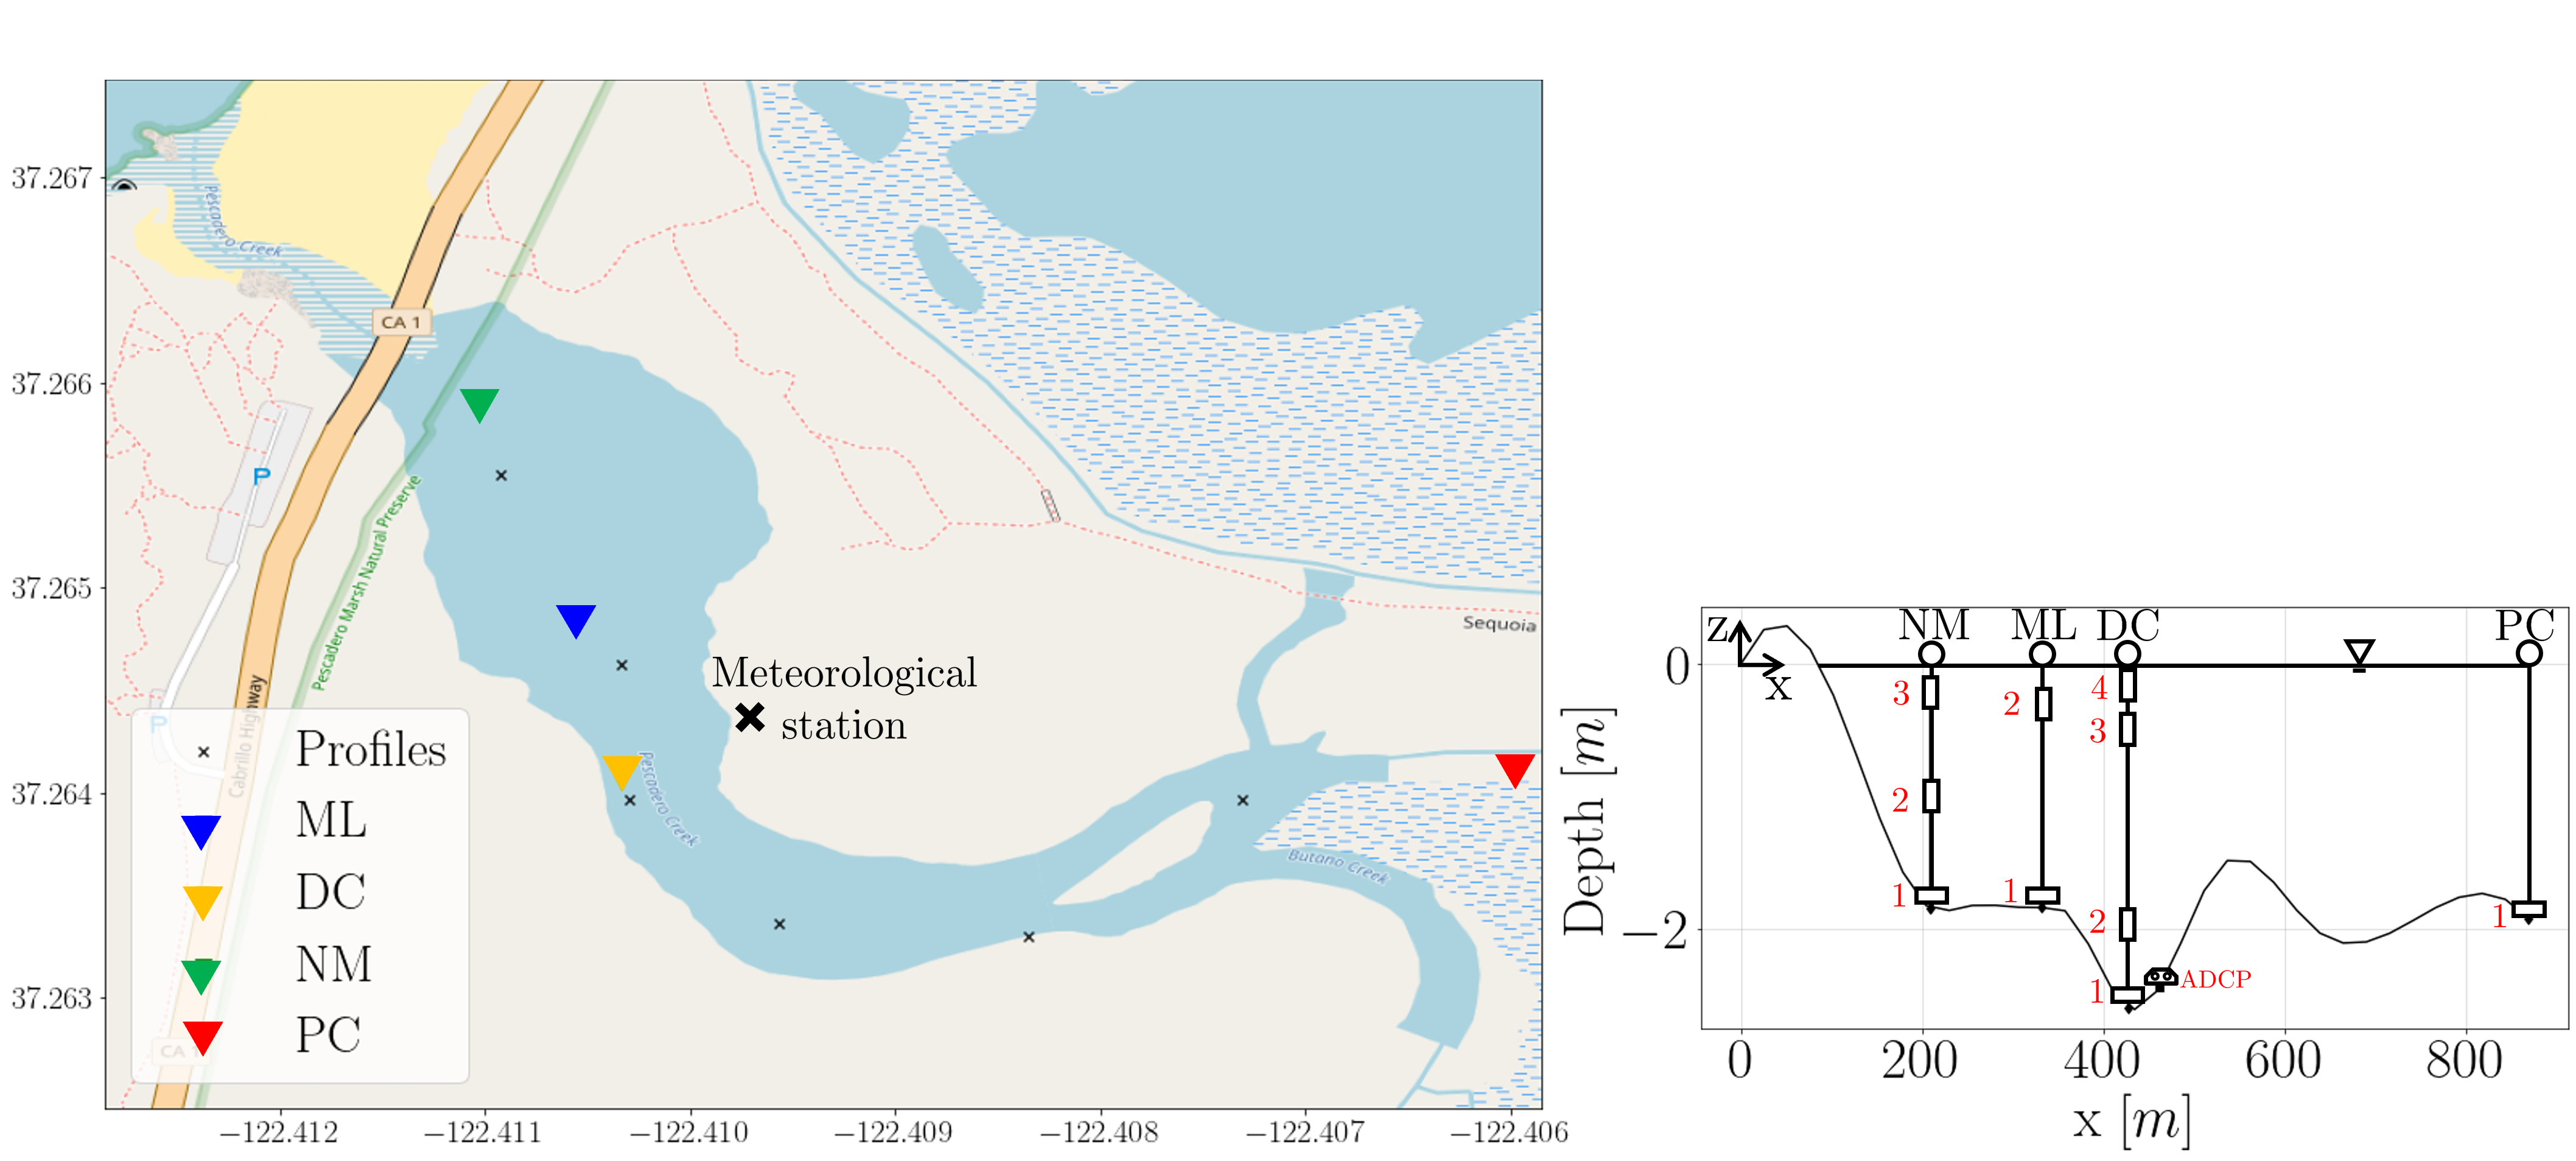
\includegraphics[width=\textwidth]{Imagenes/mapa3.png}
    \caption{Pescadero estuary map and location of the moorings (NM: Near Mouth, ML: Mid-Lagoon, DC: Deep Channel and, PC: Pescadero Creek), meteorological station. Profile locations for CTD measurements in Fig. \ref{fig:mapPDO} are indicated by small "x". Diagram of the elevation view of Pescadero in the along-estuary direction with the locations of the sensors in the water column.}
    \label{fig:mapPDO}
\end{figure}

\begin{figure}[h!]
    \centering
    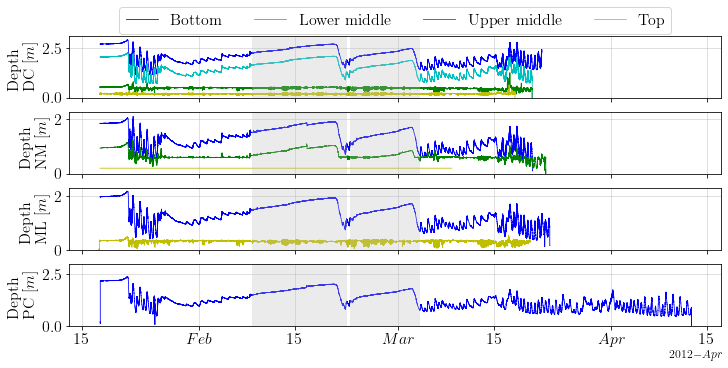
\includegraphics[width=\textwidth]{Imagenes/depth.png}
    \caption{Time-series of instruments depth in all locations. The windowed data is the used in this study.}
    \label{fig:depth}
\end{figure}

Density profiles were made on February 16th with a CTD logger around 5 p.m. at the locations indicated in Fig. \ref{fig:mapPDO}. The moment the profiles were made the wind was calm, so is not causing a disturbance in the water.\\

Velocity measurements were made with an Acoustic Doppler Current Profiler (ADCP 1200 KHz WH) anchored to the bottom of the estuary at location DC. This instrument is designed to be used in deeper water, so data collected from the surface could be affected by the interference caused by reflection. Also, this instrument, despite it is on the location DC, does not have the same depth than the CTD moored at the same location, due to the bathymetry (See diagram of Fig. \ref{fig:mapPDO}).\\

For wind speed data, an anemometer (Model $\#$05106, RM Young) was installed 3 m above the water level in marshy land adjacent to the estuary (Fig. \ref{fig:mapPDO}). All the information of the instruments are summarized in Table \ref{tab:instr}.\\


\begin{table}[h!]
    \centering
    \caption{Information of the instruments used in the field campaign.}
    \begin{tabular}{|cc|c|c|c|c|}
    \hline
    \multicolumn{2}{|c|}{Location}                & Instrument & Sampling Rate & Height above bed & Dates of data           \\ \hline
    \multicolumn{1}{|c|}{\multirow{3}{*}{NM}} & 1 & RBR XR-420 CTD    & 10 s          & 0 cm             & 17/01/2012 - 20/03/2012 \\ \cline{2-6} 
    \multicolumn{1}{|c|}{}                    & 2 & RBR XR-420 CTD    & 30 s          & 50 cm - 90 cm    & 17/01/2012 - 22/03/2012 \\ \cline{2-6} 
    \multicolumn{1}{|c|}{}                    & 3 & RBR XR-420 CTD    & 30 s          & 75 cm -  1.7 m   & 17/01/2012 - 08/03/2012 \\ \hline
    \multicolumn{1}{|c|}{\multirow{5}{*}{DC}} & 1 & RBR XR-420 CTD    & 10 s          & 0 cm             & 17/01/2012 - 21/03/2012 \\ \cline{2-6} 
    \multicolumn{1}{|c|}{}                    & 2 & RBR XR-420 CTD    & 10 s          & 50 cm - 80 cm    & 17/01/2012 - 20/03/2012 \\ \cline{2-6} 
    \multicolumn{1}{|c|}{}                    & 3 & RBR XR-420 CTD    & 10 s          & 1 m - 2 m        & 17/01/2012 - 20/03/2012 \\ \cline{2-6} 
    \multicolumn{1}{|c|}{}                    & 4 & RBR XR-420 CTD    & 10 s          & 1.3 m - 2.6 m    & 17/01/2012 - 18/03/2012 \\ \cline{2-6} 
    \multicolumn{1}{|c|}{} & \multicolumn{1}{c|}{1} & \multicolumn{1}{c|}{ADCP} & 2 Hz & \multicolumn{1}{c|}{0 m} & \multicolumn{1}{c|}{16/02/2012 - 14/03/2012} \\ \hline
    \multicolumn{1}{|c|}{\multirow{2}{*}{ML}} & 1 & RBR XR-420 CTD    & 10 s          & 0 cm             & 17/01/2012 - 20/03/2012 \\ \cline{2-6} 
    \multicolumn{1}{|c|}{}                    & 2 & RBR XR-420 CTD    & 10 s          & 40 cm - 1.6 m    & 17/01/2012 - 23/03/2012 \\ \hline
    \multicolumn{1}{|c|}{PC}                  & 1 & RBR XR-420 CTD    & 30 s          & 0 cm             & 17/01/2012 - 12/04/2012 \\ \hline
    \multicolumn{2}{|c|}{Profiles}               & RBR CTD    & 6 Hz          & -                & 16/02/2012              \\ \hline
    \multicolumn{2}{|c|}{Met. station}               & Model \# 05106, RM Young    & 6 min          & -                & 27/10/2011 - 19/04/2012  \\ \hline
    \end{tabular}
    \label{tab:instr}
    \end{table}

\subsection{External data}

To complete the information, the freshwater streamflow into the Pescadero estuary is estimated based on a United States Geological Survey (USGS) gauge located on Pescadero Creek 8.5 km upstream from the estuary mouth (USGS 11162500). As the Butano creek is also contributing, the total discharge estimation given by \cite{Williams2014} is $Q_{T} = 1.76 Q_{P,C}$. \\

The tide height data in San Francisco Bay and Monterrey Bay (stations 9414290 and 9413450 respectively) were obtained from the National Oceanographic and Atmospheric Administration (NOAA). Wave climate data were obtained from the National Data Buoy Center, 40 km offshore from the coast of Half Moon Bay (station 46012) (Fig. \ref{fig:mapext}). 

\begin{figure}[h!]
    \centering
    \includegraphics[width=0.4\textwidth]{Imagenes/mapa_ext.png}
    \caption{Stations and sites locations of the external data obtained for this study.}
    \label{fig:mapext}
\end{figure}

\subsection{Data processing}

\subsubsection{Salinity and temperature}

The CTDs measurements were made with a frequency of 10 or 30 sec, and at each location, there were one (PC), two (ML), three (NM), or four (DC) instruments at different depths (Table \ref{tab:instr}). The bottom pressure measurements at each sensor were corrected for sea-level atmospheric pressure measured at the nearest weather station located at the Half Moon Bay airport. This work focuses exclusively on the two periods where the estuary is closed between February and March.\\

We subjected the data to quality control, where data from the beginning and end, when the instrument was out of the water, and some data in the middle, where we observed time jumps incompatible with reality, were eliminated. Density is calculated from salinity, temperature, and pressure data, by the GSW Python package which is an implementation of the Thermodynamic Equation of Seawater (TEOS-2010).\\

Additionally, CTD profiles were made on February 16th, between 17:00 and 17:30 which were used to calculate the density also using TEOS-2010. When the profiles were taken the wind was very calm so we can say that the estuary was not having any significant external forcing. \\

\subsubsection{Water velocity} \label{Estuary_currents}

Velocity data collected with the ADCP in its raw form had some measured points out of the water and were in the instrument coordinates. First, we removed the data above the surface from the record and then rotated it to earth coordinates (East, North) using the method shown in \cite{teledyne2008}. On the other hand, the ADCP has a blank space of measures at the bottom, so the first measured point was 71 cm above the ground, meaning there is only a window of velocity data in the water column.\\

For a better analysis, velocity data collected with the ADCP were axis-rotated to the principal coordinates ($u,v$), based on its direction of maximum variance as shown in Fig. \ref{fig:rotacion}. This was calculated for the studied period, obtaining an angle of $48.6^o$ from the west axis in a clockwise direction and we established that the velocity was positive in the direction of the flow ($u$), that is, towards the sea.  

\begin{figure}[h!]
    \centering
    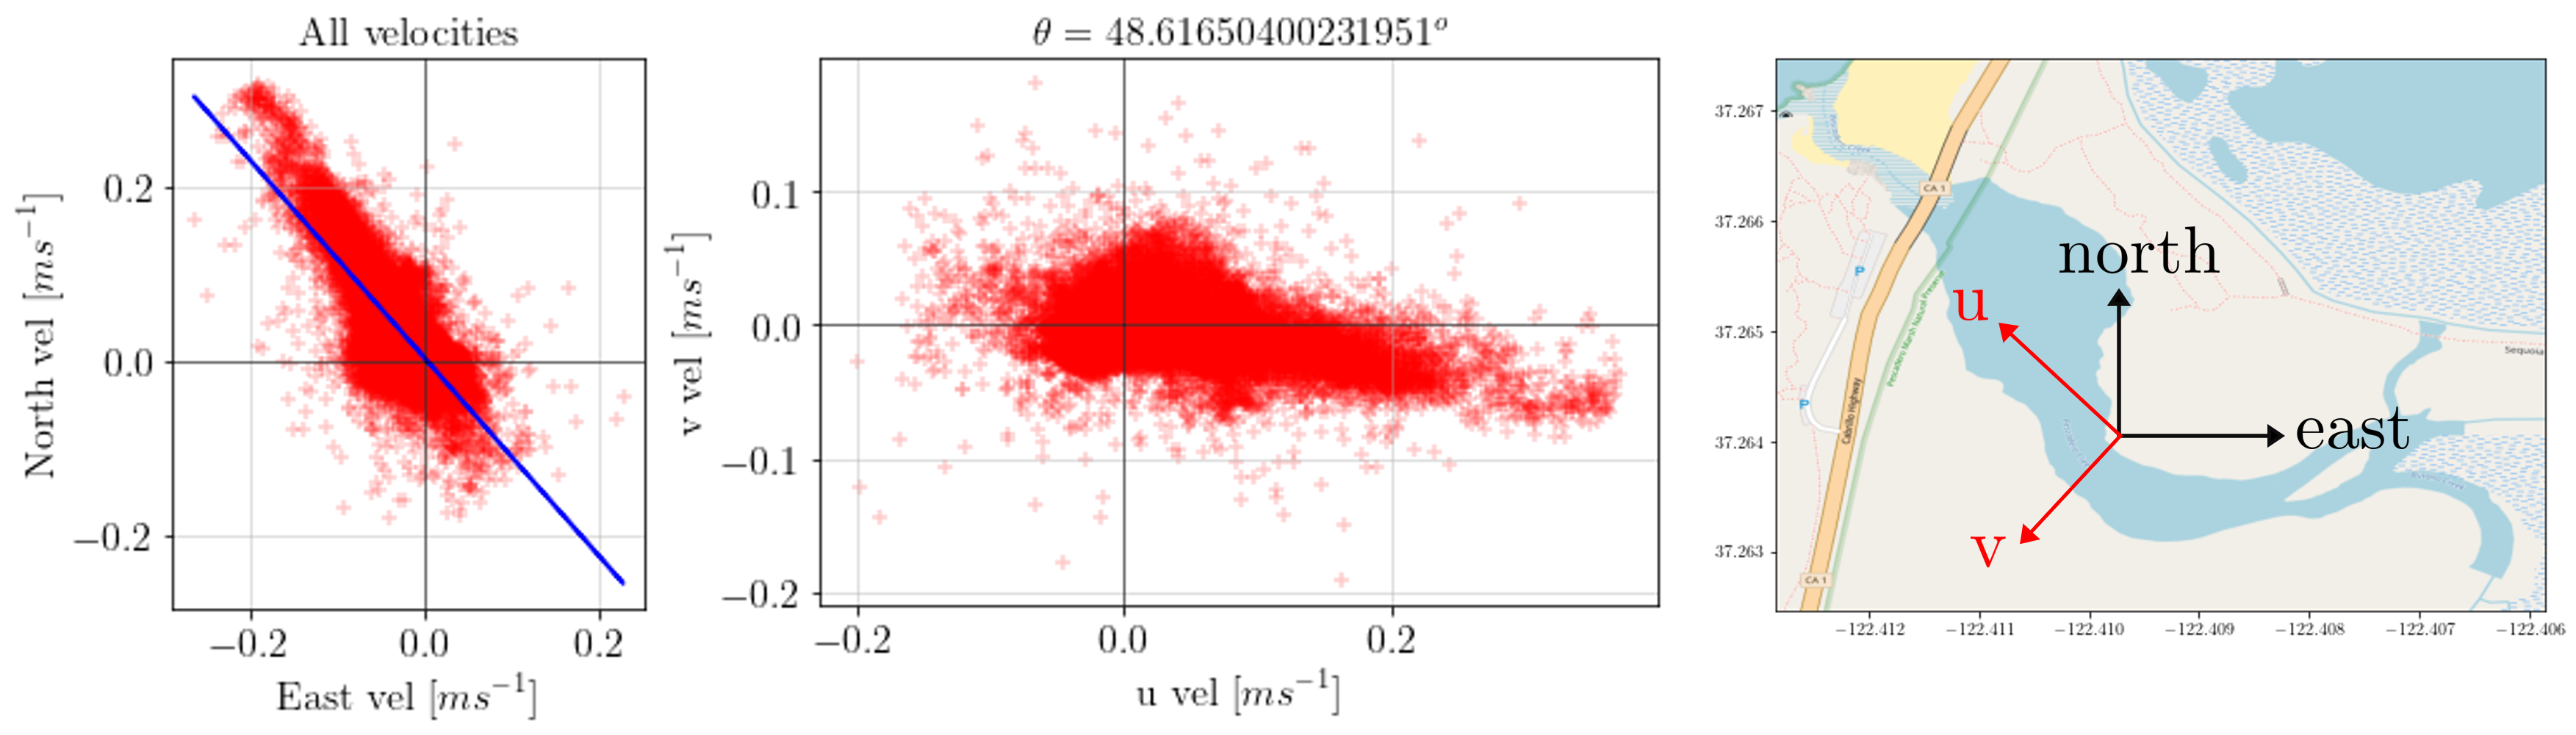
\includegraphics[width=\textwidth]{Imagenes/rotacion.png}
    \caption{Velocity data plotted in North-East and $u-v$ coordinates, and a map of Pescadero signaling the coordinates.}
    \label{fig:rotacion}
\end{figure}

We averaged ADCP data every 5 minutes to take off high-frequency signals. However, CTD data at the DC location was not at the same depth due to bathymetry so, we estimated the difference between both and adjusted the first cell to 0.91 m above the bottom of the estuary. 

\subsubsection{Wind velocity}

Raw wind data contained the velocity magnitude and direction as shown in Fig. \ref{fig:wind_raw}. Directions between 300 and 360 degrees come from the ocean and the wind that blows from 100 to 170 degrees comes from inland. Wind velocity coordinates were transformed first in east-north coordinates. Then, the data were also axis-rotated to the principal coordinates of the estuary currents, with an angle of $48.6^o$.

\begin{figure}[h!]
    \centering
    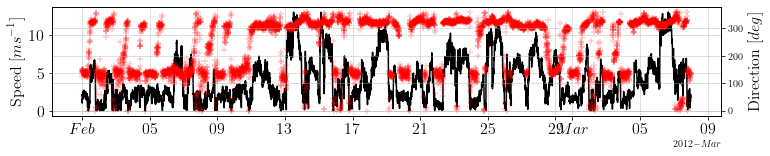
\includegraphics[width=\textwidth]{Imagenes/wind_raw.png}
    \caption{Time-series of wind velocity magnitude and direction.}
    \label{fig:wind_raw}
\end{figure}

\subsection{Analysis techniques}

\subsubsection{Stratification}

To represent stratification we used buoyancy frequency, defined as \citep{kundu2002fluid}:

\begin{equation}
    N^2 = -(g/\rho)(\partial \rho/\partial z)
    \label{eq: N2}
\end{equation}

where $\rho$ is the density of the fluid, $g$ is $9.81 m/s^2$ and $z$ is the depth. This equation is representing the water column stability, which increases or decreases as the fluid is more or less stratified. The potential energy anomaly was calculated to observe the behavior of density in the water column. It represents the work per volume required to completely mix the water column and is calculated using the equation shown by \cite{simpson1990tidal}: 

\begin{equation}
    \phi=\frac{1}{h}\int^h_0(\bar{\rho}-\rho)gzdz
    \label{eq: phi}
\end{equation}

where $h$ is the total depth, and which we discretized according to the number of sensors that each location had and considering each layer's limits as the corresponding upper and lower sensors and the density for the whole layer as the upper one. We employed the potential energy anomaly ($\phi$) as a diagnostic tool to assess the stratification of the water column before and after a wind event, thereby characterizing the state of the water column under conditions of zero wind stress and investigating the presence of mixing. Furthermore, we calculated the buoyancy frequency ($N^2$) during wind events to examine its relationship with density and velocity profiles.

\subsubsection{Wind stress}

We calculated the wind shear stress above the surface using the equation from \cite{read2011derivation}: 

\begin{equation}
    \tau=\rho_{air} C_D U_{10}^2
    \label{eq: tau}
\end{equation}

Where $\rho_{air}$ is the specific weight of air (1.2 $kg/m^3$), $C_D$ is the drag coefficient and was defined by \cite{large1981open} at 0.0012 for wind velocities between 4 and 11 m/s, and considering that the collected speeds are smaller than 11 m/s and the results are not sensitive to $C_D$ it was set as 0.0012. $U_{10}$ is the adjusted wind speed at 10 meters high, and it was obtained by: 

\begin{equation}
    U_{10}^2=U_z*(1-\frac{C_D}{\kappa}*\ln{\frac{10}{z}})^{-1}
    \label{eq: adjvel}
\end{equation}

with $\kappa=0.4$ as the Von Karmann coefficient and z = 3 m.\\

To study the response of the stratified layers to a wind impulse and identify the upwelling we used the Wedderburn number \citep{Shintani2010}:

\begin{equation}
    W=\frac{g'*h_1^2}{L*u_*^2}
    \label{eq: wed}
\end{equation}

where we estimated $h_1$ as the 30\% of the DC's total depth, L as 392 m, and for $u_*$ and g' we used:

\begin{equation}
    g'=\frac{\rho_{bottom}-\rho_{surface}}{\rho_{surface}}*g
    \label{eq: redg}
\end{equation}

\begin{equation}
    u_*^2=\frac{\tau_w}{\rho_{surface}}
    \label{eq: ustar}
\end{equation}


To analyze the relationship between wind stress and density we standardized and normalized the signals and applied cross-correlation. Cross-correlation between wind stress and density signals is used to find the time lag (phasing) between both and their level of correlation along the locations (propagation) measured in the estuary. Also, we can compare the results to the response tilt time that can be considered as $1/4$ of the internal wave period $T_1$ \citep{stevens1996initial}: 

\begin{equation}
    T_1=\frac{2L}{\sqrt{(\frac{\epsilon g h_1 h_2}{h_1 + h_2})}}
    \label{eq: period}
\end{equation}

\subsubsection{Surface fluctuations analysis}

To analyze what was happening on the surface, a frequency spectral analysis was carried out in order to identify the most important processes that affect the water level. First, \cite{welch1967use} method was applied to reduce the data noise and there was applied a detrend. Finally, the signal was multiplied by a quadratic window $w[n]=\left( \frac{n-N/2}{N/2} \right)^2$, $0 \leq n \leq N$ to obtain much clearer data and then apply the frequency spectral analysis. \\

To complement this information, an analysis of the wavelet transform was carried out using the Python package PyWavelets \citep{lee2019pywavelets}. The one-dimensional continuous wavelet transform was applied to the DC surface height data using the first-order Gaussian derivative family for a period range between 10 s and 2.8 min, we limited the frequencies to highlight what is important. This, in order to identify important events and other external phenomena, such as a wave overtopping the sandbar due to high tide. This analysis delivers coefficients that are a function of scale and position and that serve as a scalogram to visualize the wavelet.\\

To carry out a more detailed visual analysis, the standardized heights were obtained at the NM and DC points, first applying a linear detrend and then dividing the data by the standard deviation. This is for comparing results on the same scale. All the mentioned data were plotted according to local time, to analyze visually considering the factors that affect day and night as temperature and wind.

\end{document}